\section{Physical model}
\label{sec:model}

In order to present the mathematical model of the ball and plate system,
Figure~\ref{fig:model} shows the $xz$ view of the coordinate system,
introducing the needed parameters to define.
The $yz$ view is identical to the $xz$ view,
considering $\hat{y}$, $y$, $\dot{y}$, $\ddot{y}$, $\theta_y$,
$\omega_y$, $\dot{\omega}_y$ in place of $\hat{x}$, $x$, $\dot{x}$,
$\ddot{x}$, $\theta_x$, $\omega_x$ and $\dot{\omega}_x$, respectively.
Hence, the $yz$ view is omitted.

The sizes of the ball and plate system (in millimeters) are reported in
Table~\ref{tab:measurements}.

Although the real system presents the vertical axes $H$ split in two parts,
as far as we are concerned the proposed model is still valid.
More precisely, the rotation joint is located along the $H$ segment, which means
that it does not coincide with the plate center which in turn is not a fixed
point anymore, causing a greater $\theta$ for the same $alpha$.

A servomotor is in charge of imposing the angle $\alpha$ which,
through the joint $h$, moves the plate of an angle $\theta$.
The forces, which acts on the ball, are the friction and weight forces.

\begin{figure}[htb]
  \centering

  \psfrag{x}[bc]{\small$\hat{x}$}
  \psfrag{z}[bc]{\small$\hat{z}$}
  \psfrag{plate}[bc]{\small$plate$}

  \psfrag{v}[bc]{\small$x, \dot{x}, \ddot{x}$}
  \psfrag{o}[bc]{\small$\theta, \dot{\omega}, \ddot{\omega}$}

  \psfrag{alpha}[bc]{\small$\alpha$}
  \psfrag{tetha}[bc]{\small$\theta$}
  \psfrag{phi}[bc]{\small$\gamma$}

  \psfrag{H}[bc]{\small$H$}
  \psfrag{D}[bc]{\small$D$}
  \psfrag{r}[bc]{\small$r$}
  \psfrag{b}[bc]{\small$b$}
  \psfrag{h}[bc]{\small$h$}
  \psfrag{l}[bc]{\small$l$}
  \psfrag{r}[bc]{\small$r$}
  \psfrag{R}[bc]{\small$R$}

  \psfrag{mg}[bc]{\small$m\overline{g}$}
  \psfrag{F}[bc]{\small$\overline{F}$}
  \psfrag{N}[bc]{\small$\overline{N}$}

  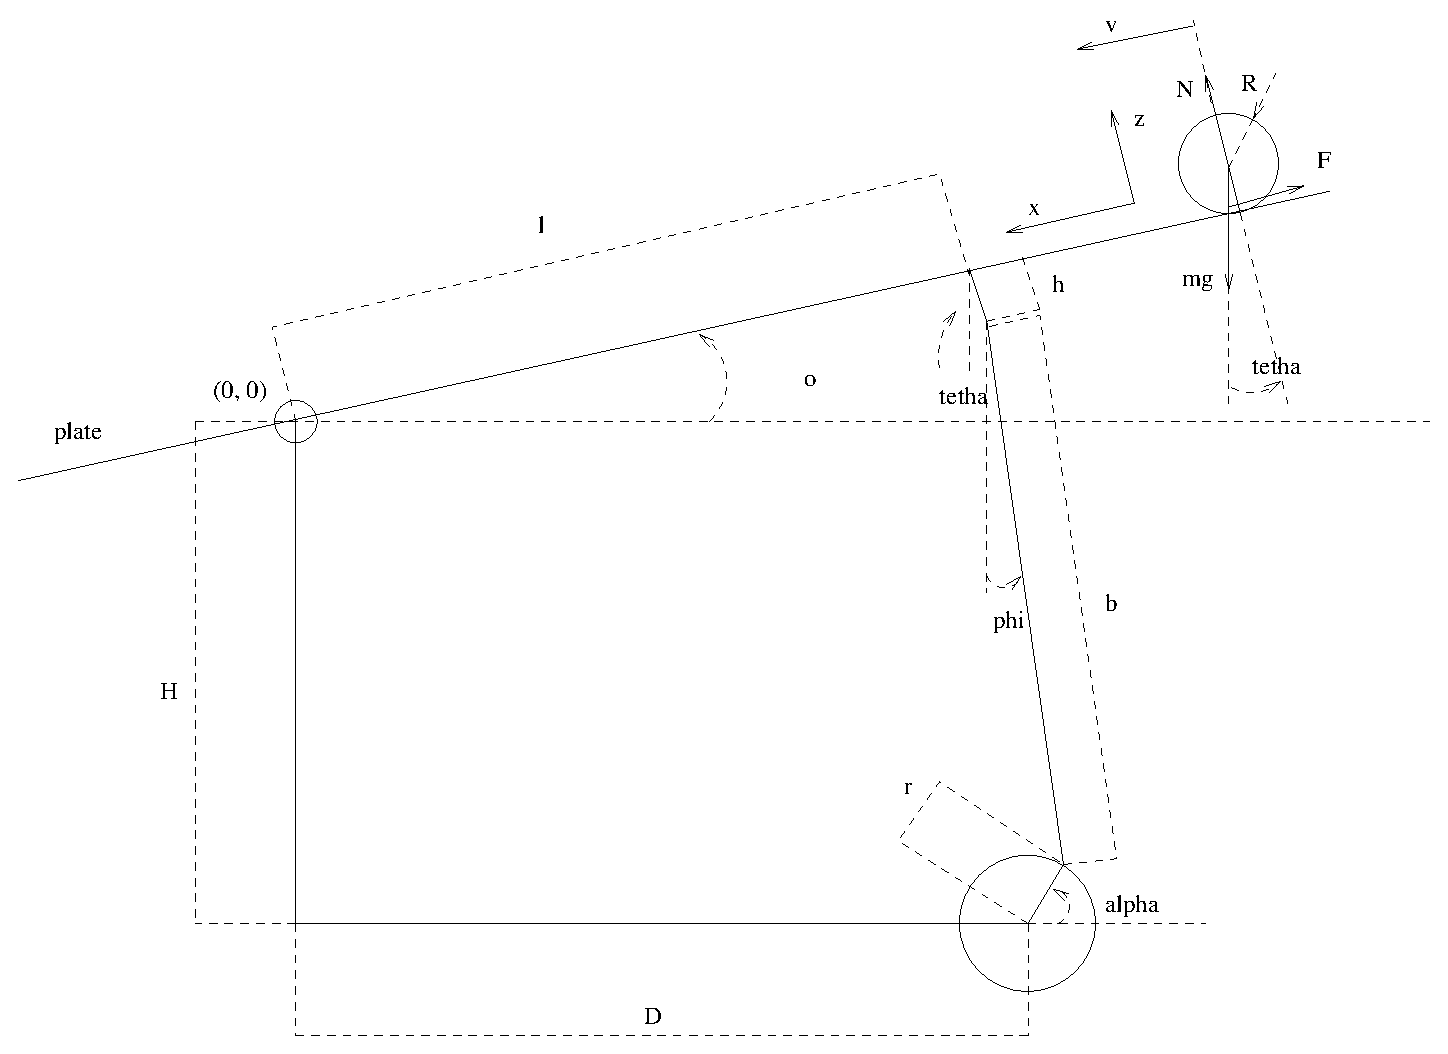
\includegraphics[width=0.9\columnwidth]{model}
  \caption{Physical model.}
  \label{fig:model}
\end{figure}

\begin{table}
	\centering
	\begin{tabular}{ |c|c|c|c|c|c|c|c|c| }
		\hline
		$l_x$ & $l_y$ & $D_x$ & $D_y$ & $H_x$ & $H_y$ & $h$ & $b$ & $r$\\
		\hline
		76    & 62    & 66.5  & 53    & 47    & 49    & 16  & 40  & 20\\
		\hline
	\end{tabular}
	\caption{Plate measurements (mm).}
	\label{tab:measurements}
\end{table}

